\newpage
\section{Profilo utente}

\subsection{Gestione profilo}

Una volta effettuato il login, è possibile accedere al proprio profilo utente. La schermata principale relativa al profilo apparirà come nella figura sottostante.

\label{Profilo utente}
\begin{figure}[H]
	\centering
	\fbox{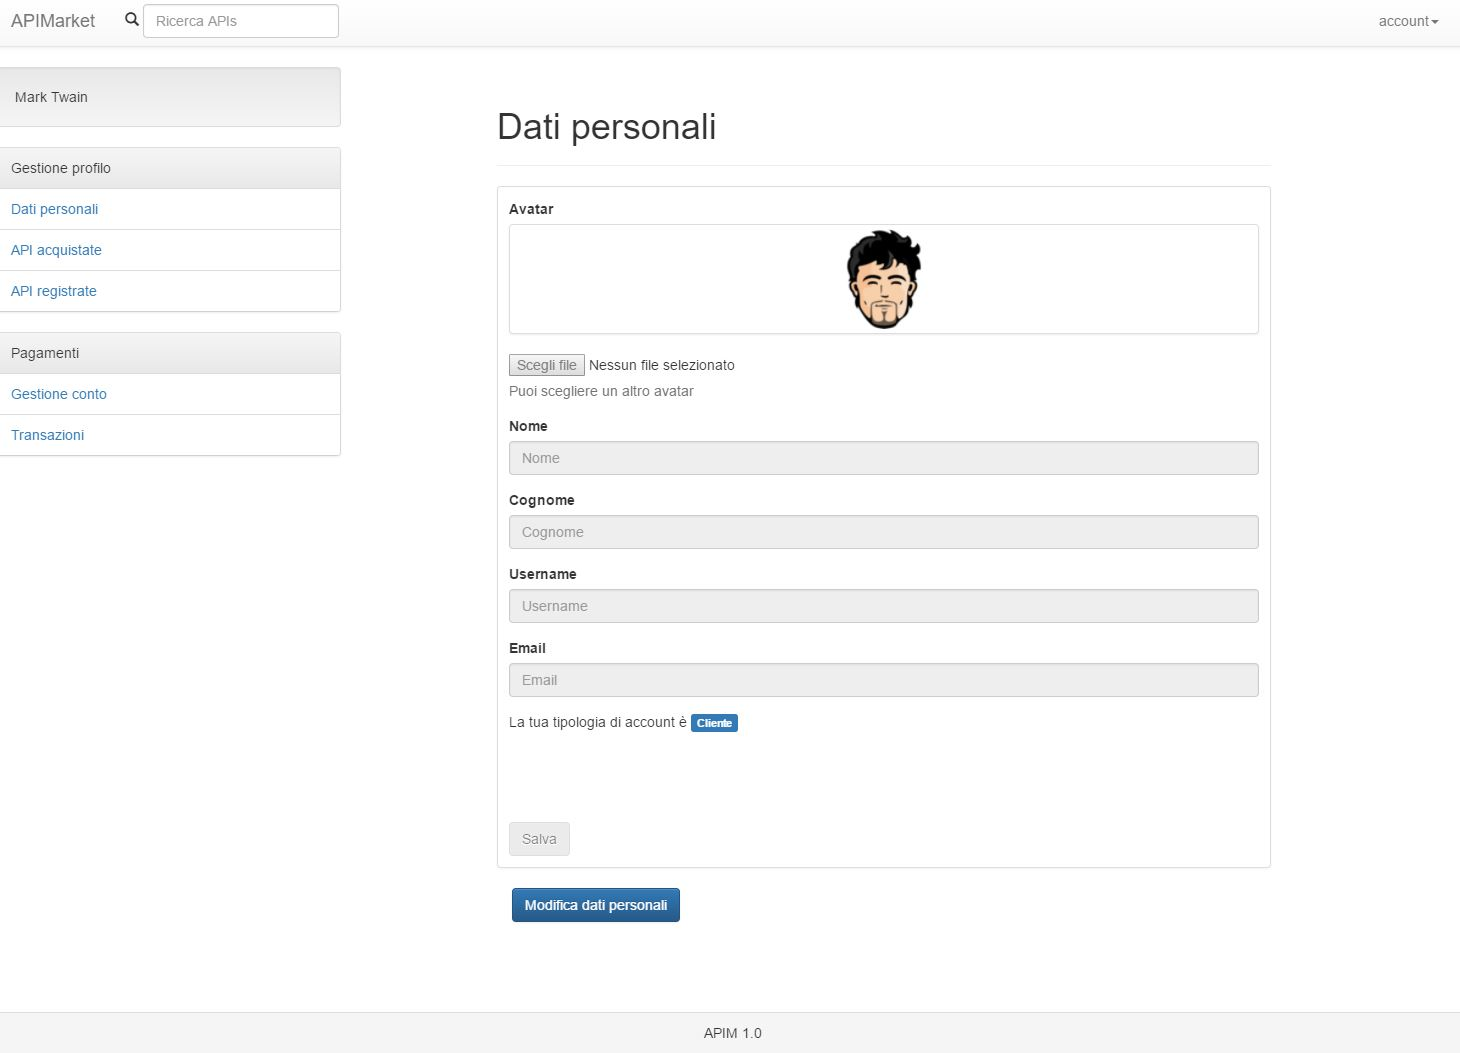
\includegraphics[scale=0.52]{img/APIM_account.JPG}}
	\caption{Profilo utente}
\end{figure}

Dalla schermata si potranno modificare i dati personali, inseriti al momento della registrazione, quali la propria anagrafica o dati relativi all'account quali l'immagine personale. E' visualizzato inoltre a quale gruppo di utenza si appartiene: l'utente registrato semplice infatti è un utente denominato "cliente", mentre l'utente abilitato al caricamento e alla vendita di servizi è denominato utente "sviluppatore".

Tramite il menù laterale è possibile navigare nelle schermate del proprio profilo. Clickando sulla voce API acquistate si potrà consultare l'elenco delle api attualmente in possesso o acquistate in passato con i relativi dati. 

\label{API acquistate}
\begin{figure}[H]
	\centering
	\fbox{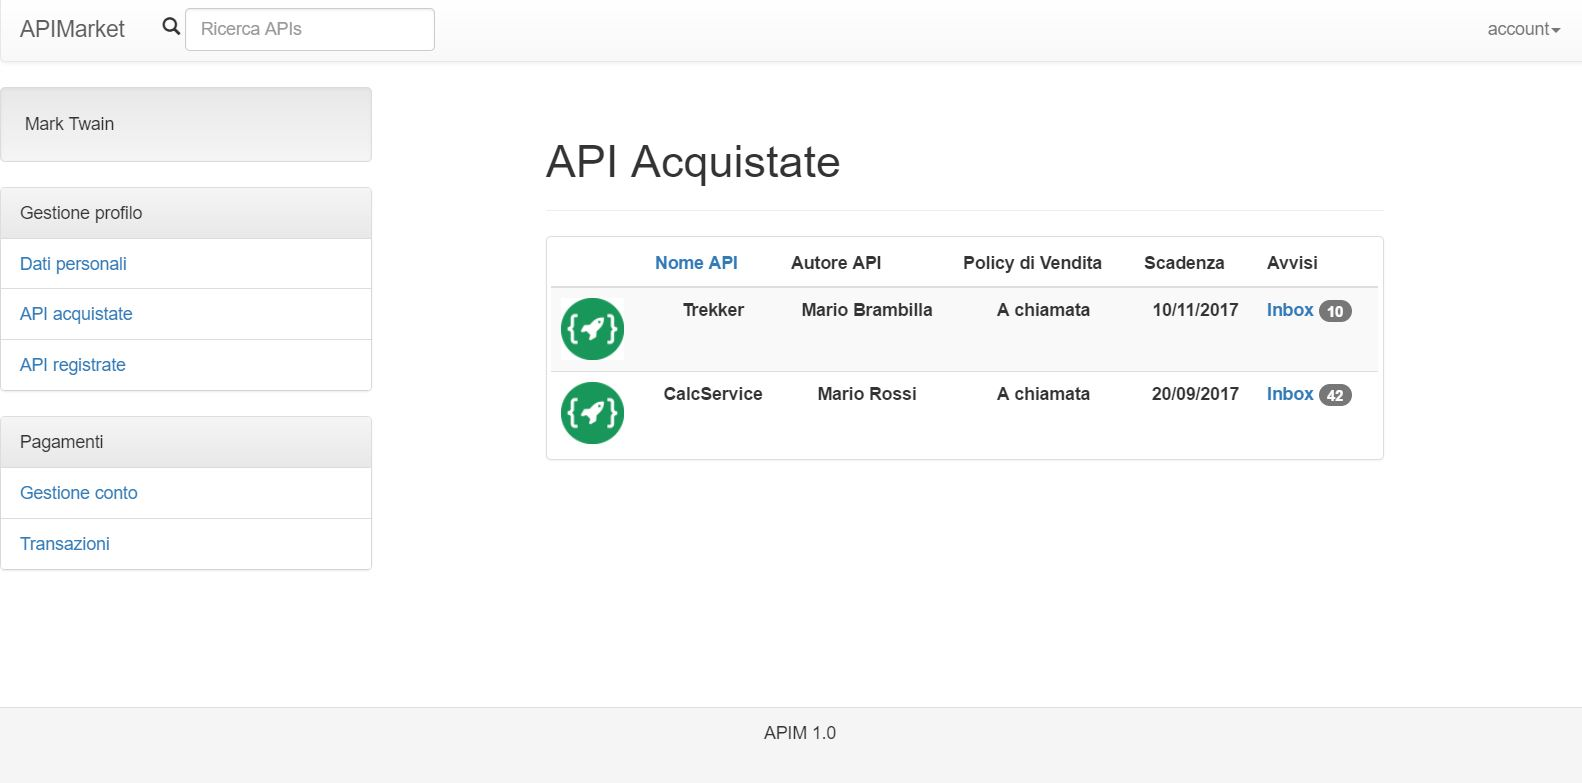
\includegraphics[scale=0.47]{img/APIM_apiAcquistate.JPG}}
	\caption{API acquistate}
\end{figure}

Qualora l'utente appartenga alla categoria "sviluppatore", è disponibile la voce relativa alle API registrate con relative statistiche.

\label{API registrate}
\begin{figure}[H]
	\centering
	\fbox{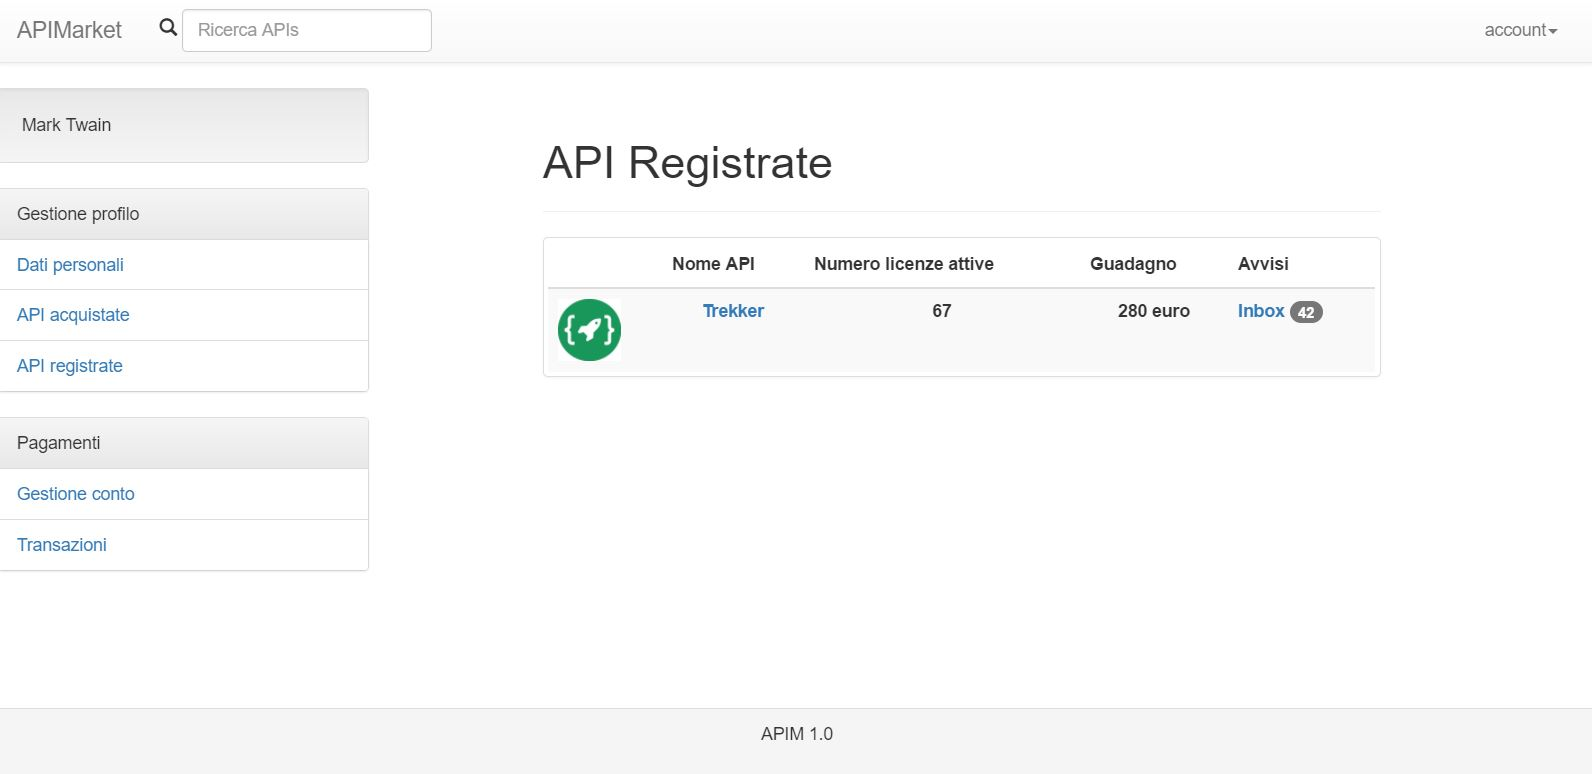
\includegraphics[scale=0.47]{img/APIM_apiRegistrate.JPG}}
	\caption{API registrate}
\end{figure}

\subsection{Registrazione API}

L'utente abilitato alla vendita (Sviluppatore) può  registrare le proprie API per la vendita nell'apposita pagina accessibile dal profilo utente. La schermata per la registrazione di nuove API appare come mostrato nell'immagine sottostante.

\label{Registrazione API}
\begin{figure}[H]
	\centering
	\fbox{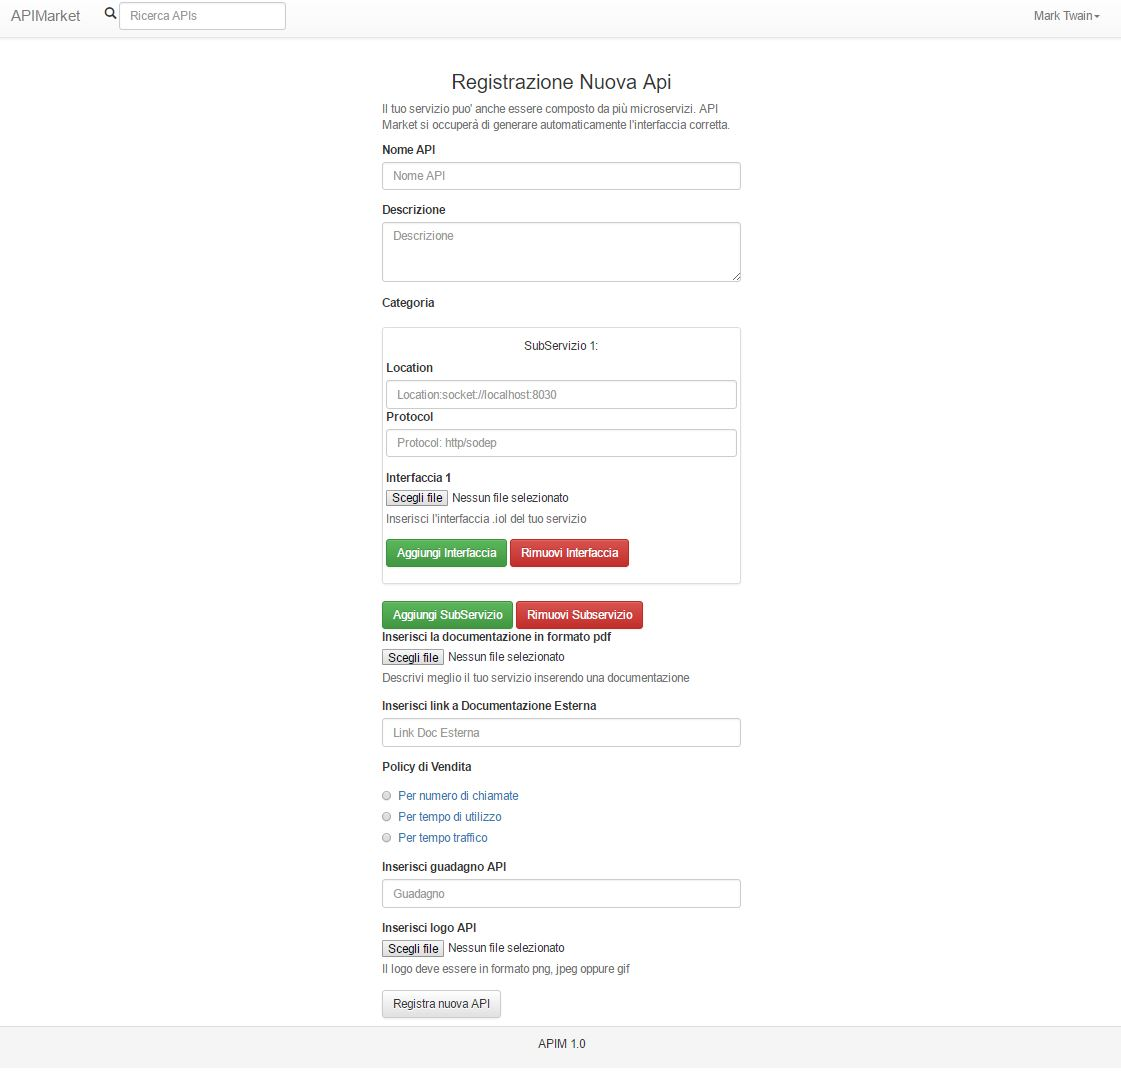
\includegraphics[scale=0.65]{img/APIM_nuovaApi.JPG}}
	\caption{Registrazione API}
\end{figure}

All'interno, l'utente dovrà specificare obbligatoriamente i seguenti dati per permettere l'inserimento del proprio prodotto nella piattaforma

\begin{itemize}
	\item Nome dell'API;
	\item Breve descrizione;
	\item Tags che identificano le categorie a cui appartiene;
	\item L'URI/Posizione del servizio;
	\item Il protocollo di comunicazione utilizzato;
	\item I file che caratterizzano l'interfaccia;
	\item Posizione, protocollo e interfaccia di eventuali sottoservizi correlati (opzionale);
	\item Documentazione PDF o link esterno;
	\item Il guadagno desiderato e la policy scelta;
	\item Il logo del prodotto.
\end{itemize}

Qualora i campi inseriti fossero corretti, il sistema segnala che la procedura è andata a buon fine.

\subsection{Pagamenti}

Gli utenti sviluppatori possono consultare i propri dati finanziari, quali movimenti o saldo, nelle sezioni preposte del proprio profilo. La sezione Gestione conto mostra il saldo attuale e offre la possibilità di caricare il proprio saldo tramite funzionalità esterne (PayPal).

\label{Gestione conto}
\begin{figure}[H]
	\centering
	\fbox{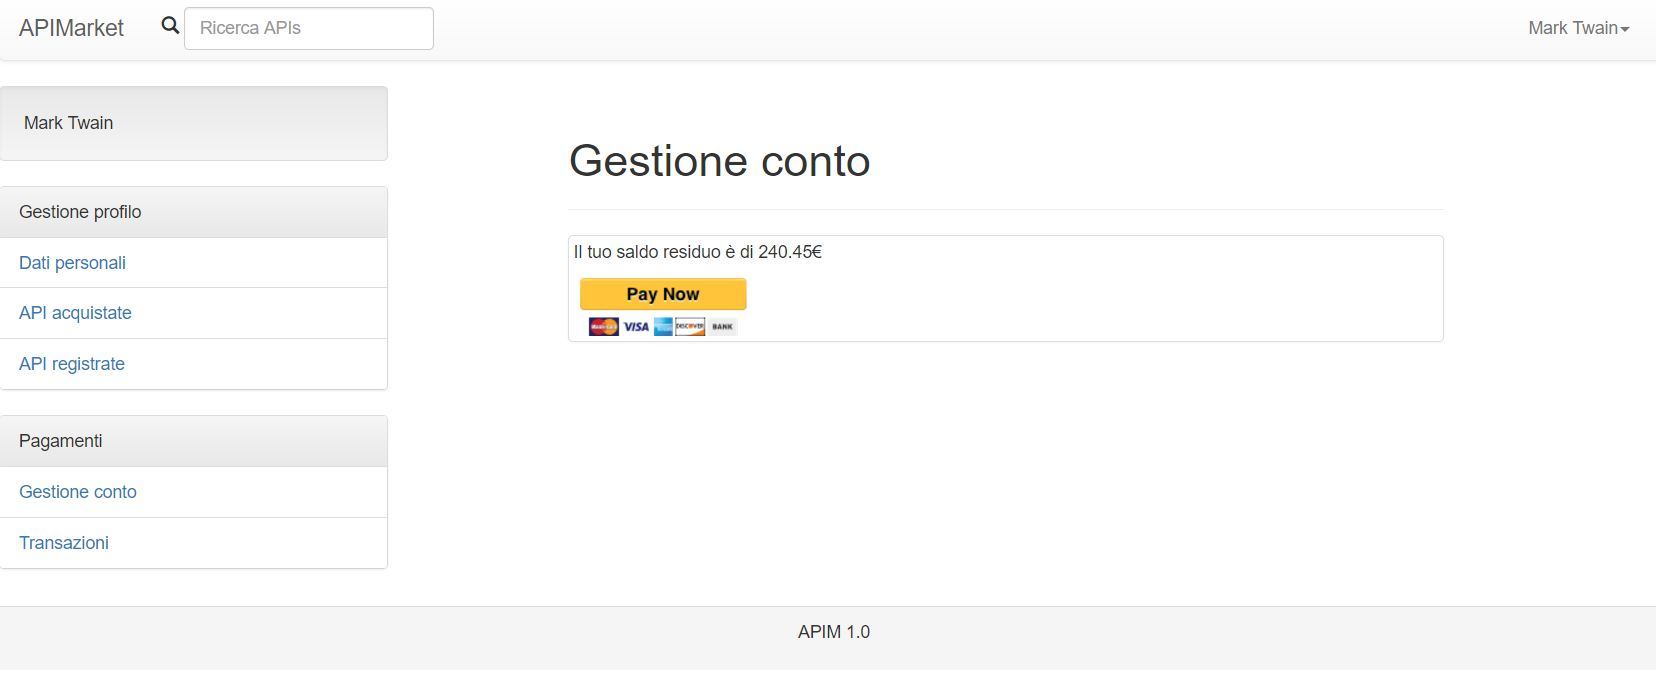
\includegraphics[scale=0.45]{img/APIM_gestioneConto.JPG}}
	\caption{Gestione conto}
\end{figure}

Nella voce transazioni, invece, è disponibile uno storico delle transazioni effettuate nell'API Market. Esse riguardano i servizi utilizzati e le relative chiamate, o gli addebiti per policy di altra tipologia. Lo storico contiene la designazione dell'API che è stata utilizzata, il costo, e la data. Esiste inoltre un ID univoco della transazione, per poter referenziare una particolare transazione con lo staff API Market.

\label{Transazioni}
\begin{figure}[H]
	\centering
	\fbox{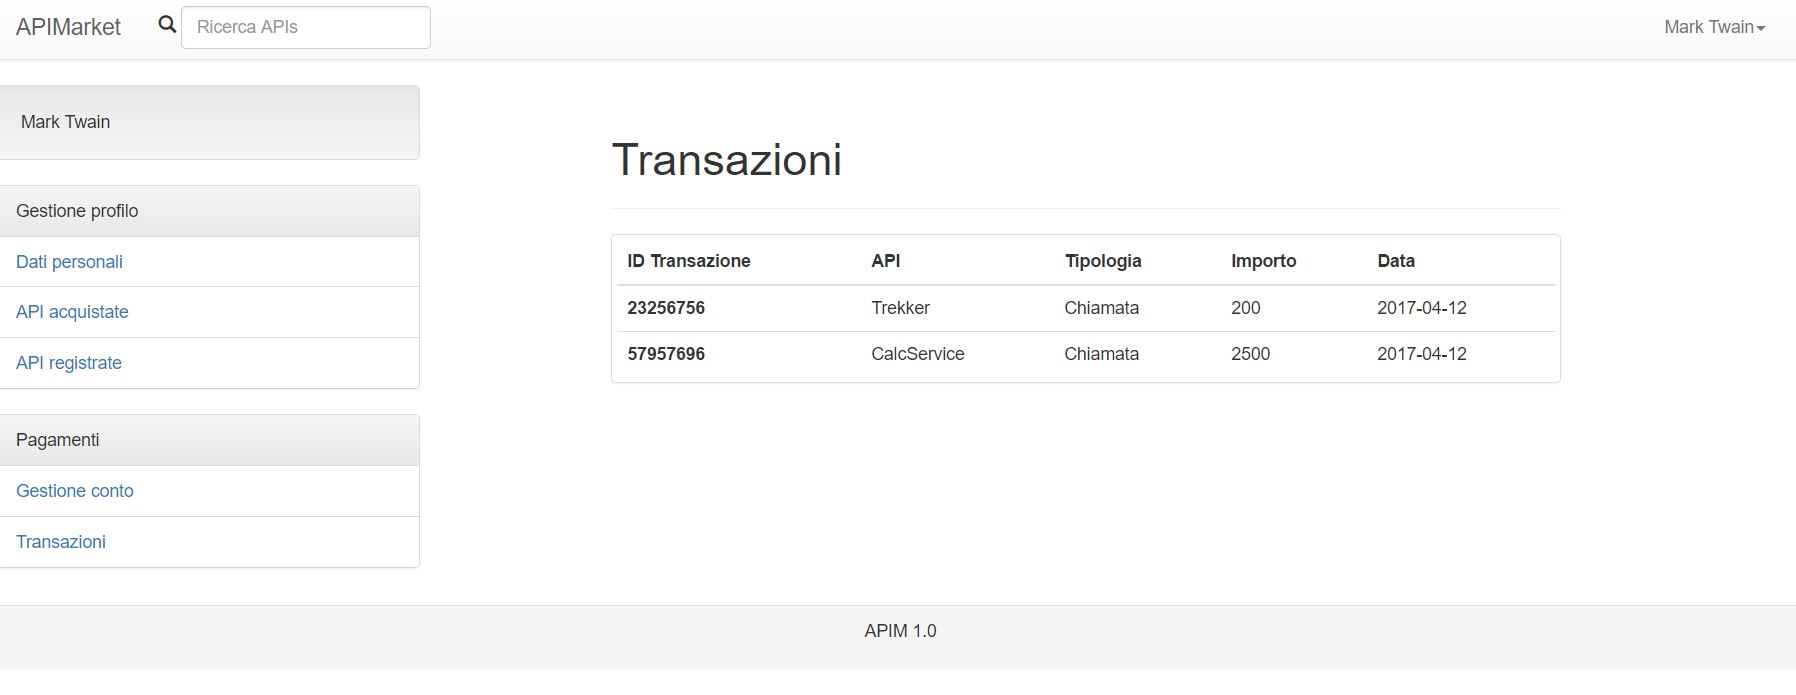
\includegraphics[scale=0.42]{img/APIM_transazioni.JPG}}
	\caption{Transazioni}
\end{figure}